\documentclass[abstract=on, letterpaper]{scrartcl}
\usepackage[onehalfspacing]{setspace}

\usepackage[version=3]{mhchem} % Package for chemical equation typesetting
\usepackage{mathabx} %Astronomical symbols
\usepackage{siunitx} % Provides the \SI{}{} and \si{} command for typesetting SI units
\usepackage{graphicx} % Required for the inclusion of images
\usepackage{subfigure}
\usepackage{natbib} % Required to change bibliography style to APA
\usepackage{amsmath} % Required for some math elements 
\usepackage[german, english]{babel} % Deutsch für Umlaute
\usepackage{etoolbox}
\usepackage{tabularx}
\newcolumntype{R}{>{\raggedleft\arraybackslash}X}
\apptocmd{\UrlBreaks}{\do\f\do\m}{}{}
\usepackage{framed}
%\usepackage[utf8]{luainputenc}
\usepackage[T1]{fontenc}
\usepackage{floatrow}
\usepackage{blindtext}
\usepackage[bottom]{footmisc}
\usepackage{tablefootnote}
\setlength\parindent{7pt} % Removes all indentation from paragraphs

\usepackage[backref]{hyperref}
\hypersetup{backref=true, pagebackref=true, hyperindex=true, breaklinks=true,colorlinks=true,urlcolor=blue, linkcolor=blue,  citecolor=blue, bookmarks=true, bookmarksopen=true}
\usepackage{natbib}
\bibpunct{(}{)}{;}{a}{}{,}

\usepackage{geometry}
\geometry{letterpaper, left=2cm, right=2cm, top=2.5cm, bottom=2.5cm}
\usepackage{xcolor}
%\usepackage{amsfonts}
\renewcommand{\labelenumi}{\alph{enumi}.} % Make numbering in the enumerate environment by letter rather than number (e.g. section 6)

%Setzt den equation-Zaehler nach jeder Seite zurueck
\numberwithin{equation}{section}

\DeclareSIUnit\year{yr}
\DeclareSIUnit\parsec{pc}

%Definiert den Stil:
\renewcommand{\theequation}{\arabic{section}.\arabic{equation}}

\selectlanguage{english}

\title{Desiccation of the Trappist-1 Planets}
\subtitle{Draft 0.0}
\author{Patrick Barth}

\date{\today}

\begin{document}
	
	
\maketitle
		
\tableofcontents
\newpage

%-----------------------------------------------------------

\section{Introduction}

%The goal of this report is to summarize the work I have done during the first two phases of my research project, the scientific specialization (MFS) and methods and project planning (MFP).
%The MFS I have completed at the University of Washington, Seattle, together with Rory Barnes in the Virtual Planet Laboratory (VPL) from January to June 2018.
%The MFP includes my work at the MPIA since September 2018 under the supervision of Prof. Thomas Henning and Dr. Ludmila Carone.
%
%The goal of my research project is to write a code that simulates the interaction between the atmosphere and the molten mantle (magma ocean) of an exoplanet and to implement this model into the VPLanet code of the VPL.
%Basis for this model is the coupled atmosphere interior-model by \citet{Schaefer2016}.
%
%In Section \ref{Sec_Model} I will present the model from \citet{Schaefer2016}.
%A time consuming part of my thesis was the calculation of the atmospheric net flux that leads to the cooling of the planet.
%I will discuss this part in detail in Section \ref{Sec_Flux}.


\section{The Model}
\label{Sec_Model}

%The idea behind this model is the following:
%After its formation the planet is very hot such that the mantle is molten.
%During its evolution the planet cools and the magma ocean starts to solidify from the bottom of the mantle to the surface of the planet.
%The model by \citet{Schaefer2016} consists of two parts: 
%The thermal model calculates the evolution of the temperature of the magma ocean and the solidification radius.
%The volatile model keeps track of the water and oxygen contents in the individual reservoirs (atmosphere, magma ocean, and solidified mantle).
%Figure \ref{struc_magma} shows the structure of the mantle during the solidification.

\begin{figure}[H]
	\label{struc_magma}
	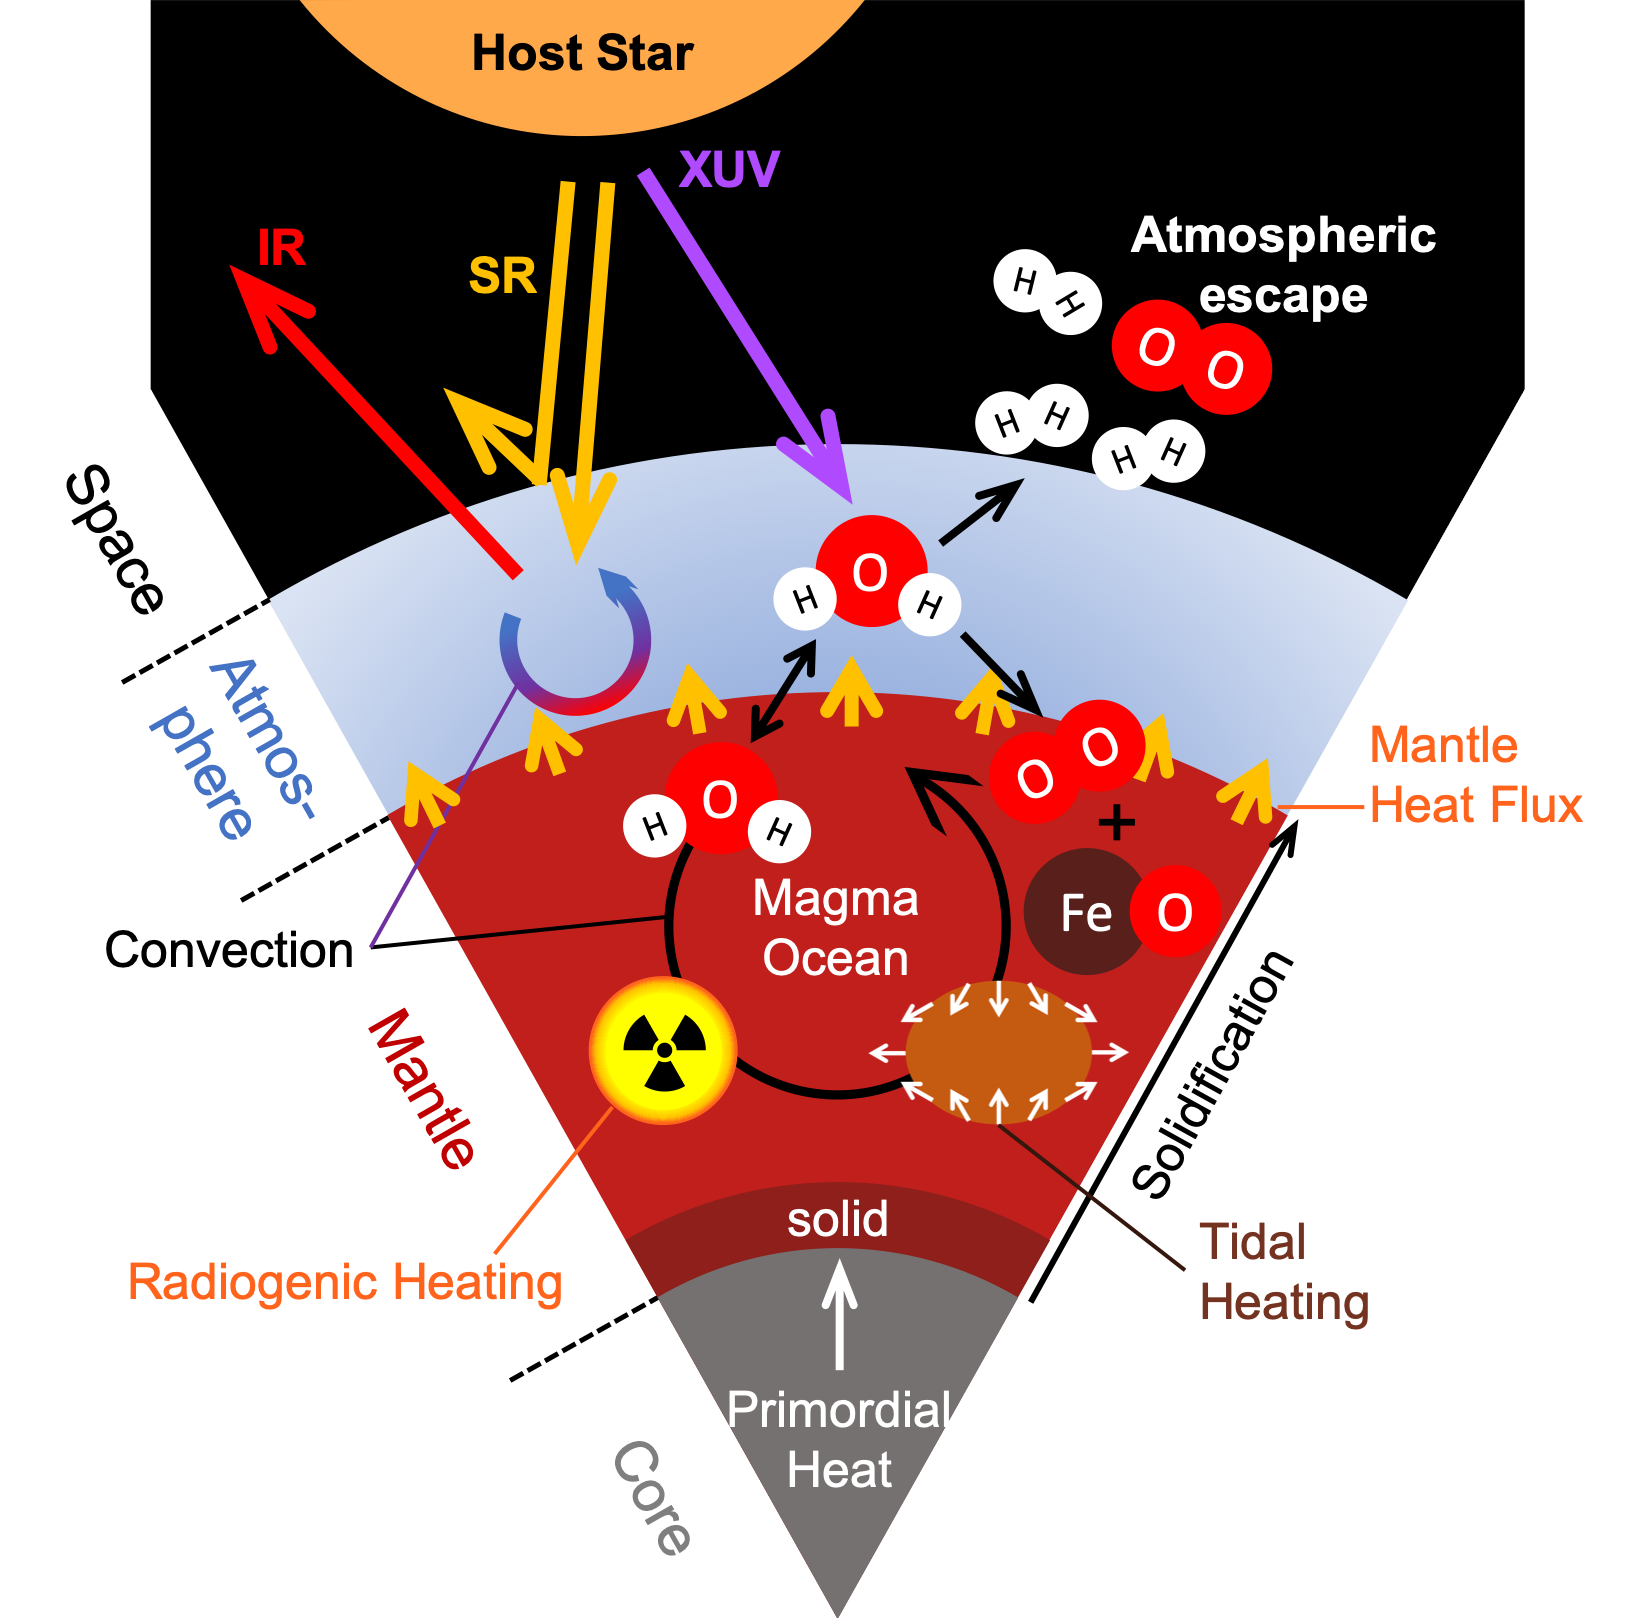
\includegraphics[width=0.6\textwidth]{../Fig_StructMagmaOcean/struc_magma}
	\caption{Structure of the magma ocean at a time step during the solidification process. $r_\mathrm{p}$ is the radius of the planet, at $r_\mathrm{l}$ the temperature equals the liquidus temperature, at $r_\mathrm{s}$ the solidus temperature, and $r_\mathrm{b}$ is the bottom of the initially molten magma ocean. From \citet{Lebrun2013}.}
\end{figure}

%\subsection{Thermal Model}
%
%The thermal model returns the potential temperature $T_\mathrm{p}$, the surface temperature $T_\mathrm{surf}$, and the solidification radius $r_\mathrm{s}$ for every time step.
%In addition, it keeps track of the melt fraction $\psi$ and the time derivative of $r_\mathrm{s}$ for the volatile model. The initial parameters are $T_\mathrm{p} = T_\mathrm{surf} = \SI{4000}{\kelvin}$ and $r_\mathrm{s} = r_\mathrm{c}$, where $r_\mathrm{c}$ is the core radius.
%
%The thermal model is governed by two differential equations which describe the change of the surface and the potential temperature:
%\begin{eqnarray}
%	\label{Deriv_Tpot}
%	\frac{4}{3} \pi \rho_\mathrm{m} c_\mathrm{p} (r^3_\mathrm{p} - r^3_\mathrm{s}) \frac{dT_\mathrm{p}}{dt}     &=& 4 \pi r^2_\mathrm{s} \Delta H_\mathrm{f} \rho_\mathrm{m} \frac{dr_\mathrm{s}}{dt} - 4 \pi r^2_\mathrm{p} q_\mathrm{m} + \frac{4}{3} \pi \rho_\mathrm{m} Q_\mathrm{r} (r^3_\mathrm{p} - r^3_\mathrm{c}) \\
%	\left( c_{\mathrm{p},\ce{H2O}} M_\mathrm{atm} +  c_\mathrm{p,m} \frac{4}{3} \pi \rho_\mathrm{m} (r^3_\mathrm{p} - \delta^3) \right) \frac{dT_\mathrm{surf}}{dt} &=& 4 \pi r^2_\mathrm{p} (q_\mathrm{m} - \mathcal{F})
%\end{eqnarray}
%A list of the used parameters including their values is provided in table \ref{Tab_Therm_Model}, the parameters of the planet GJ1132b can be found in table \ref{Tab_Param_GJ1132b}.
%$g$ is the gravitational acceleration at the surface.
%\begin{center}
%	\begin{table}[H]
%	\begin{tabular}{ccc}
%		\noalign{\smallskip}
%		\hline
%		\noalign{\smallskip}
%		Symbol & Parameter & Value \\ 
%		\noalign{\smallskip}
%		\hline \hline
%		\noalign{\smallskip}
%		$\rho_\mathrm{m}$ & Mantle bulk density & $\SI{4000}{\kilogram\per\cubic\metre}$\\ 
%		$c_\mathrm{p} $ & Silicate heat capacity & $1.2 \times 10^3 \SI{}{\joule\per\kilogram\per\kelvin}$ \\
%		$\Delta H_\mathrm{f}$ & Heat of silicate fusion & $4 \times 10^5 \SI{}{\joule\per\kilogram}$ \\
%		$q_\mathrm{m}$ & Mantle heat flux & \\
%		$Q_\mathrm{r}$ & Heat generated by radioactive decay & \\
%		$c_{\mathrm{p},\ce{H2O}} $ & Heat capacity of water &\\
%		$\mathcal{F}$ & Heat flux leaving the atmosphere & OLR - ASR\footnote{OLR = Outgoing Longwave Radiation, ASR = Absorbed Stellar Radiation}\\
%		$\delta$ &Thickness of the thermal boundary layer & $k (T_\mathrm{p} - T_\mathrm{surf}) / q_\mathrm{m} $\\
%		$k$ & Thermal conductivity & $\SI{4.2}{\watt\per\metre\per\kelvin}$\\
%		$\alpha$ & Thermal expansion coefficient & $2 \times 10^{-5} \SI{}{\per\kelvin}$ \\
%		$\kappa$ & Thermal diffusivity & $10^{-6} \SI{}{\metre\squared\per\second}$ \\
%		$\nu$ & Kinematic viscosity &\\
%		$Ra_\mathrm{cr}$ & Critical Raleigh number & $1.1 \times 10^3$ \\
%		\noalign{\smallskip}
%		\hline
%	\end{tabular}
%	\caption{Parameters for the thermal model}
%	\label{Tab_Therm_Model}
%	\end{table}
%\end{center}
%
%\begin{center}
%	\begin{table}[h]
%		\begin{tabular}{ccc}
%			\noalign{\smallskip}
%			\hline
%			\noalign{\smallskip}
%			Symbol & Parameter & Value \\ 
%			\noalign{\smallskip}
%			\hline \hline
%			\noalign{\smallskip}
%			$r_\mathrm{p} $ & Planetary radius & $1.15 \, R_\Earth = 7.33 \times 10^6 \SI{}{\metre}$ \\
%			$M_\mathrm{p} $ & Planetary mass  & $1.62 \, M_\Earth = 9.67 \times 10^{24} \SI{}{\kilogram}$ \\
%			$r_\mathrm{c}$ & Core radius & $1.15 \, r_{\mathrm{c},\Earth} = 3.91 \times 10^6 \SI{}{\metre}$ \\
%			$A$ & Albedo (steam atmosphere)& 0.75 \\
%			\noalign{\smallskip}
%			\hline
%		\end{tabular}
%		\caption{Parameters of GJ1132b (\url{http://exoplanet.eu/catalog/gj_1132_b/})}
%		\label{Tab_Param_GJ1132b}
%	\end{table}
%\end{center}
%
%The mantle heat flux $q_\mathrm{m}$ is the heat flux that leaves the magma ocean at the surface.
%It depends on the difference between $T_\mathrm{p}$ and $T_\mathrm{surf}$.
%If $T_\mathrm{p} > T_\mathrm{surf}$, convection is cooling the mantle and $q_\mathrm{m}$ is given by
%\begin{equation}
%	q_\mathrm{m} = \frac{k (T_\mathrm{p} - T_\mathrm{surf})}{l} \left( \frac{Ra}{Ra_\mathrm{cr}} \right)^\beta.
%\end{equation}
%With the Rayleigh number defined by
%\begin{equation}
%	Ra = \frac{\alpha g (T_\mathrm{p} - T_\mathrm{surf}) l^3}{\kappa \nu}
%\end{equation}
%and $\beta = 1/3$ this combines to
%\begin{equation}
%	q_\mathrm{m} = k (T_\mathrm{p} - T_\mathrm{surf})^{4/3} \left( \frac{\alpha g}{\kappa \nu Ra_\mathrm{cr}} \right)^{1/3}.
%\end{equation}
%If $T_\mathrm{p} < T_\mathrm{surf}$, however, the convection stops and heat is transported upwards only by the conductive flux which is negligible in the first case:
%\begin{equation}
%	q_\mathrm{m,cond} = k T_\mathrm{p} \frac{\alpha g}{c_\mathrm{p}}
%\end{equation}
%The kinetic viscosity $\nu$ can be expressed with the dynamic viscosity $\eta$: $\nu = \eta / \rho_\mathrm{m}$.
%I discuss the viscosity profile of the magma ocean in section \ref{SubSec_Viscosity}.
%
%The radiogenic heating rate $Q_\mathrm{r}$ is given by \citet{Schaefer2015}
%\begin{equation}
%	Q_\mathrm{r} = \sum C_i H_i \exp \left[ \lambda_i \left( 4.6 \times 10^9 - t \right) \right],
%\end{equation}
%where $i$ is indicating the individual radioactive isotope, $C_i$ is the mantle concentration, $H_i$ the heat production per unit mass, and $\lambda_i$ the decay constant of the specific element.
%The values for these constants are taken from \citet{Turcotte2002}.
%
%\begin{center}
%	\begin{table}[h]
%		\begin{tabular}{lccc}
%			\noalign{\smallskip}
%			\hline
%			\noalign{\smallskip}
%			Element & Concentration $C$ & Heat Release $H$ & Decay constant $\lambda$ \\ 
%			 & $ (\SI{}{\kilogram\per\kilogram})$ & $ (\SI{}{\watt\per\kilogram})$ &  $ (\SI{}{\per\giga\year})$\\
%			\noalign{\smallskip}
%			\hline \hline
%			\noalign{\smallskip}
%			\ce{^{238}U} & $30.8 \times 10^{-9}$ & $9.46 \times 10^{-5}$ & $1.551 \times 10^{-1}$\\
%			\ce{^{235}U} & $0.22 \times 10^{-9}$ & $5.69 \times 10^{-4}$ & $9.846 \times 10^{-1}$\\
%			\ce{^{232}Th} & $124 \times 10^{-9}$ & $2.64 \times 10^{-5}$ & $4.951 \times 10^{-2}$\\
%			\ce{^{40}K} & $36.9 \times 10^{-9}$ & $2.92 \times 10^{-5}$ & $0.5545 \times 10^{-1}$\\
%			\noalign{\smallskip}
%			\hline
%		\end{tabular}
%		\caption{Constants for the radiogenic elements \citep{Turcotte2002}}
%		\label{Tab_Radiogenic}
%	\end{table}
%\end{center}
%
%Unlike \citet{Schaefer2016}, I don't use only the potential temperature to determine the melt fraction and the solidification radius. 
%Instead, I use $T_\mathrm{p}$ to calculate the adiabatic temperature profile of the mantle at every time step, and calculate the melt fraction and the solidification radius with this profile.
%The adiabatic temperature profile is given by
%\begin{equation}
%\label{adiabatic}
%T(r) = T_\mathrm{p} \lbrack 1 + \frac{\alpha g}{c_\mathrm{p}} (r_\mathrm{p} - r) \rbrack.
%\end{equation}
%
%The solidification radius $r_\mathrm{s}$ follows this differential equation which can be inserted into Eq. (\ref{Deriv_Tpot}):
%\begin{equation}
%	\frac{dr_\mathrm{s}}{dt} = \frac{c_\mathrm{p} (b \alpha - a \rho_\mathrm{m} c_\mathrm{p})}{g (a \rho_\mathrm{m} c_\mathrm{p} - \alpha T_\mathrm{p})^2} \frac{dT_\mathrm{p}}{dt}
%\end{equation}
%
%\subsection{Volatile Model}
%
%The volatile model uses the outputs of the thermal model to calculate the amount of oxygen and water that is restored in the atmosphere and magma ocean system (mo), and the solid mantle (sol).
%We assume that in the beginning the atmosphere contains all the water on the planet.
%Atmosphere and magma ocean are in equilibrium such that the pressure of water vapor (in Pascal) in the atmosphere determines the \ce{H2O} mass fraction in the magma ocean and vice versa:
%\begin{equation}
%	p_{\ce{H2O}} = \left( \frac{ F_{\ce{H2O}} }{ 3.44 \times 10^{-8} } \right)^{1/0.74}
%	\label{water_equi}
%\end{equation}
%The parameters of the volatile model are provided in table \ref{Tab_Volat_Model}.
%
%\begin{center}
%	\begin{table}[H]
%		\begin{tabular}{ccc}
%			\noalign{\smallskip}
%			\hline
%			\noalign{\smallskip}
%			Symbol & Parameter & Value \\ 
%			\noalign{\smallskip}
%			\hline \hline
%			\noalign{\smallskip}
%			$F_{\ce{H2O}}$ & Water mass fraction in liquid melt & \\ 
%			$M_{\ce{H2O}}^{\mathrm{mo}} $ & Water mass in the magma ocean + atmosphere system &\\
%			$M_{\ce{H2O}}^{\mathrm{cyrstal}} $ & Water mass in the crystals within the magma ocean &\\
%			$M_{\ce{H2O}}^{\mathrm{liq}} $ & Water mass in the liquid magma &\\
%			$M_{\ce{H2O}}^{\mathrm{atm}} $ & Water mass in the atmosphere &\\
%			$M_{\ce{H2O}}^{\mathrm{sol}} $ & Water mass in the solidified mantle &\\
%			$k_{\ce{H2O}}$ & partition coeff. for water between melt and solid & $0.01$\\
%			$\phi_1$ & XUV-driven atmospheric mass-loss rate of H & $[\SI{}{kg\per\metre\squared\per\second}]$\\
%			\noalign{\smallskip}
%			\hline
%		\end{tabular}
%		\caption{Parameters for the thermal model}
%		\label{Tab_Volat_Model}
%	\end{table}
%\end{center}
%
%The mass balance of the water contained in the magma ocean and atmosphere system is given by the following equation:
%\begin{equation}
%	\begin{aligned}
%		M_{\ce{H2O}}^{\mathrm{mo}} &= M_{\ce{H2O}}^{\mathrm{crystal}} + M_{\ce{H2O}}^{\mathrm{liq}} + M_{\ce{H2O}}^{\mathrm{atm}} \\
%		&= k_{\ce{H2O}} F_{\ce{H2O}} M^{\mathrm{crystal}} + F_{\ce{H2O}} M^{\mathrm{liq}} + \frac{4 \pi r_\mathrm{p}^2}{g} p_{\ce{H2O}}
%	\end{aligned}
%\end{equation}
%
%There are two sinks of water in the system: the solidification of the magma ocean which is trapping water in the solid mantle and the atmospheric escape of hydrogen and oxygen at the top of the atmosphere.
%Therefore, the water mass in the different reservoirs is governed by two differential equations, taking into account both sinks:
%\begin{eqnarray}
%	\frac{dM_{\ce{H2O}}^{\mathrm{sol}}}{dt} &=& 4 \pi \rho_\mathrm{m}  k_{\ce{H2O}} F_{\ce{H2O}} r_\mathrm{s}^2 \frac{d r_\mathrm{s}}{dt} \\
%	\frac{dM_{\ce{H2O}}^{\mathrm{mo}}}{dt} &=& - \frac{dM_{\ce{H2O}}^{\mathrm{sol}}}{dt} - 4 \pi r_\mathrm{p}^2 \phi_1 \frac{\mu_{\ce{H2O}}}{2 \mu_{\ce{H}}}
%\end{eqnarray}
%
%Due to the high XUV flux from the star the water gets dissociated and the hydrogen escapes with the escape rate $\phi_1$.
%The remaining oxygen goes into the magma ocean and oxidizes \ce{FeO} to \ce{Fe2O3}.
%At one point, the oxygen also starts to escape with the rate $\phi_2$.
%I calculate $\phi_1$ and $\phi_2$ with the atmospheric escape model by \citet{Luger2015a}.
%
%The amount of oxygen in the different reservoirs is governed by a similar set of differential equations:
%\begin{eqnarray}
%	\frac{dM_{\ce{O}}^{\mathrm{sol}}}{dt} &=& 4 \pi \rho_\mathrm{m}  F_{\ce{FeO_{1.5}}} r_\mathrm{s}^2 \frac{d r_\mathrm{s}}{dt} \frac{\mu_{\ce{O}}}{2 \mu_{\ce{FeO_{1.5}}}}\\
%	\frac{dM_{\ce{O}}^{\mathrm{mo}}}{dt} &=& 4 \pi r_\mathrm{p}^2 \left(  \phi_1 \frac{\mu_{\ce{O}}}{2 \mu_{\ce{H}}} - \phi_2 \right) - \frac{dM_{\ce{O}}^{\mathrm{sol}}}{dt}
%\end{eqnarray}
%However, unlike water which dissolves into the magma ocean following Eq. (\ref{water_equi}), the oxygen reacts with the \ce{FeO} in the magma, oxidizing it to \ce{Fe2O3}.
%This chemical process follows an empirical relation derived by \citet{Kress1991}:
%\begin{equation}
%	\begin{aligned}
%		\ln \left( \frac{X_{\ce{Fe2O3}}}{X_{\ce{FeO}}} \right) &= 0.196 \ln (f_{\ce{O2}}(\SI{}{\pascal})) + \frac{\SI{11492}{\kelvin}}{T_\mathrm{p}} - 6.675 - 2.243 X_{\ce{Al2O3}} \\
%		&- 1.828 X_{\ce{FeO}^*} + 3.201 X_{\ce{CaO}} + 5.854 X_{\ce{Na2O}} + 6.215 X_{\ce{K2O}} \\
%		&- 3.36 \left[ 1 - \frac{\SI{1673}{\kelvin}}{T_\mathrm{p}} - \ln \left( \frac{T_\mathrm{p}}{\SI{1673}{\kelvin}} \right) \right] - 7.01 \times 10^{-7} \frac{p_\mathrm{atm} (\SI{}{\pascal})}{T_\mathrm{p} (\SI{}{\kelvin})} \\
%		&- 1.54 \times 10^{-10} \frac{(T_\mathrm{p} - \SI{1673}{\kelvin}) p_\mathrm{atm} (\SI{}{\pascal})}{T_\mathrm{p}} + 3.85 \times 10^{-17} \frac{p^2_\mathrm{atm} (\SI{}{\pascal})}{T_\mathrm{p} (\SI{}{\kelvin})}
%	\end{aligned}
%\end{equation}
%It depends on the oxygen fugacity (i.e. the partial pressure of oxygen in the atmosphere), the potential temperature of the magma ocean, and the composition of the magma ocean.
%The composition used by \citet{Schaefer2016} and in my model is the Bulk Silicate Earth \citep{ONeill1998}.
%
%
%%-------------------------------------------
\section{Validation with GJ1132b}
\label{GJ1132b}

\begin{figure}[H]
	\includegraphics[width=0.8\textwidth]{../Fig_GJ1132b/SolidTime_MassFracWater_No5_ConstThermTemp_400K}
	\caption{Solidification time of GJ1132b's mantle depending on the initial water mass fraction. Results with VPLanet for three different XUV absorption efficiencies (0, 0.15, 0.3) are compared to the results from \citet{Schaefer2016} (Fig. 5).}
	\label{SolidTimeGJ}
\end{figure}

%---------------------------------------------------------------------------------%
\section{Trappist-1}

\subsection{Time Evolution}
\begin{figure}[H]
	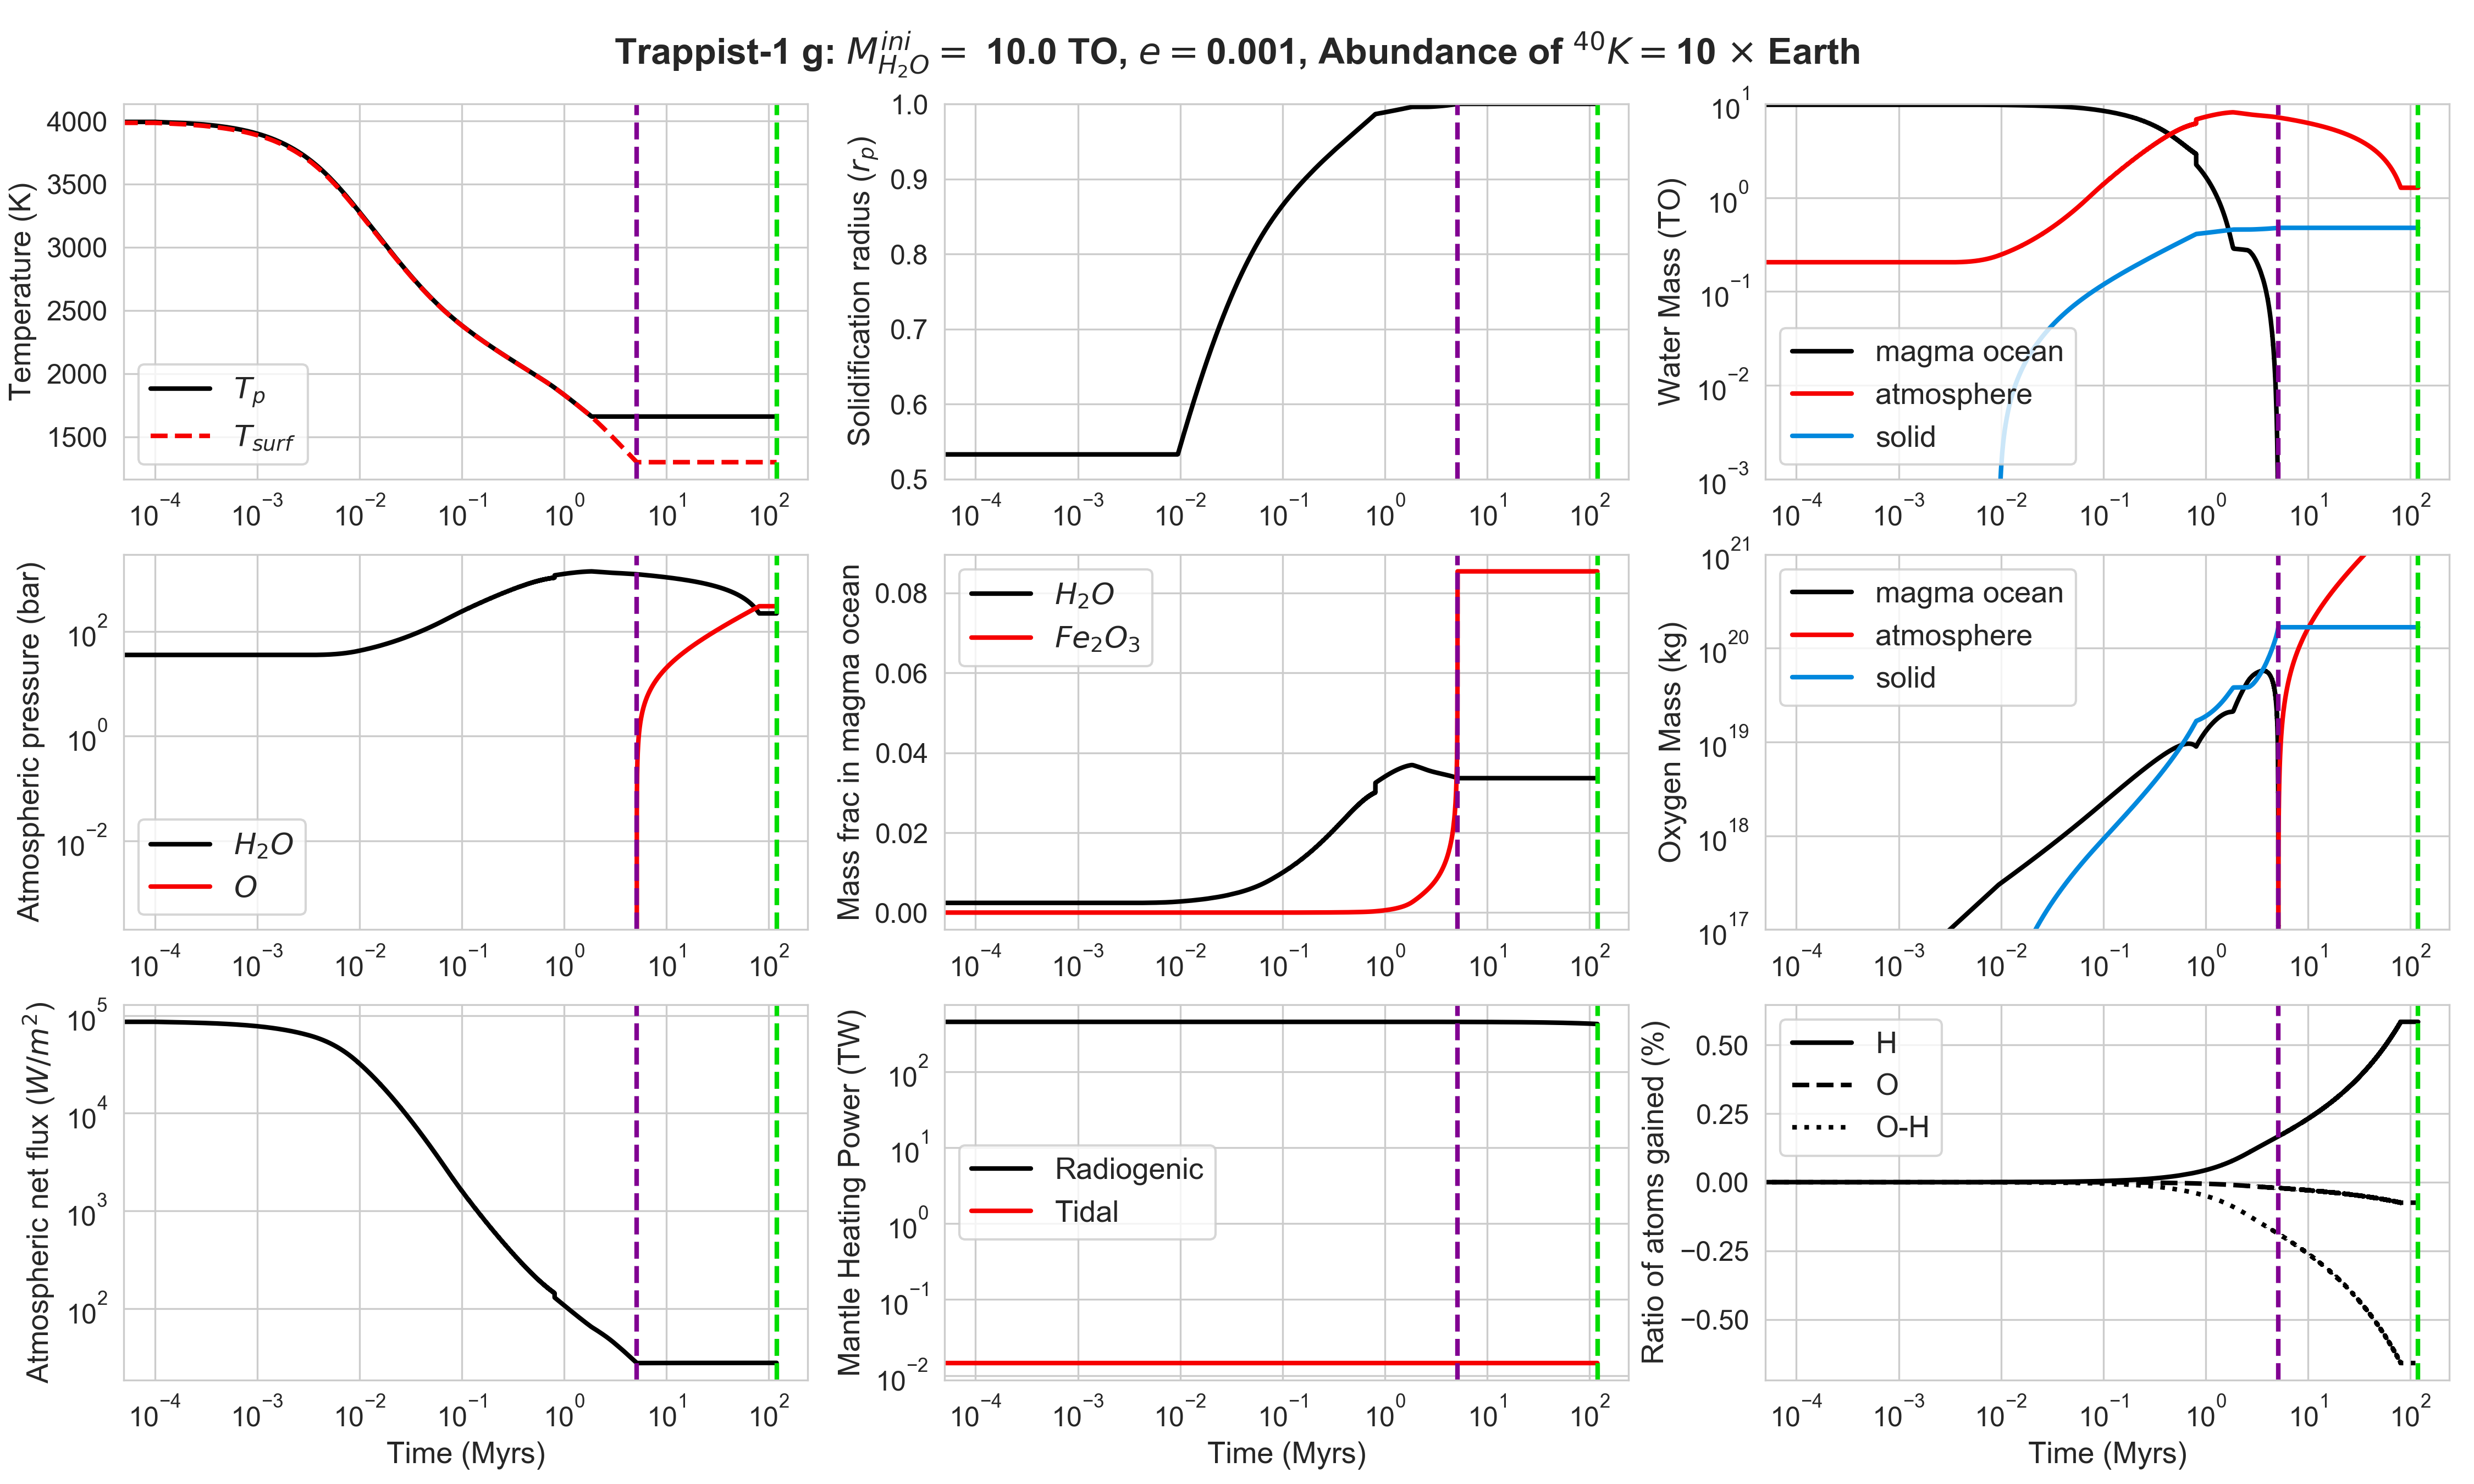
\includegraphics[width=\textwidth]{../Fig_Trappist1_TimeEvolution/Trappist-1_g_10TO_ecc_001_40K_10}
	\caption{}
	\label{TR1g_Time}
\end{figure}

\subsection{Results}

\begin{figure}[H]
	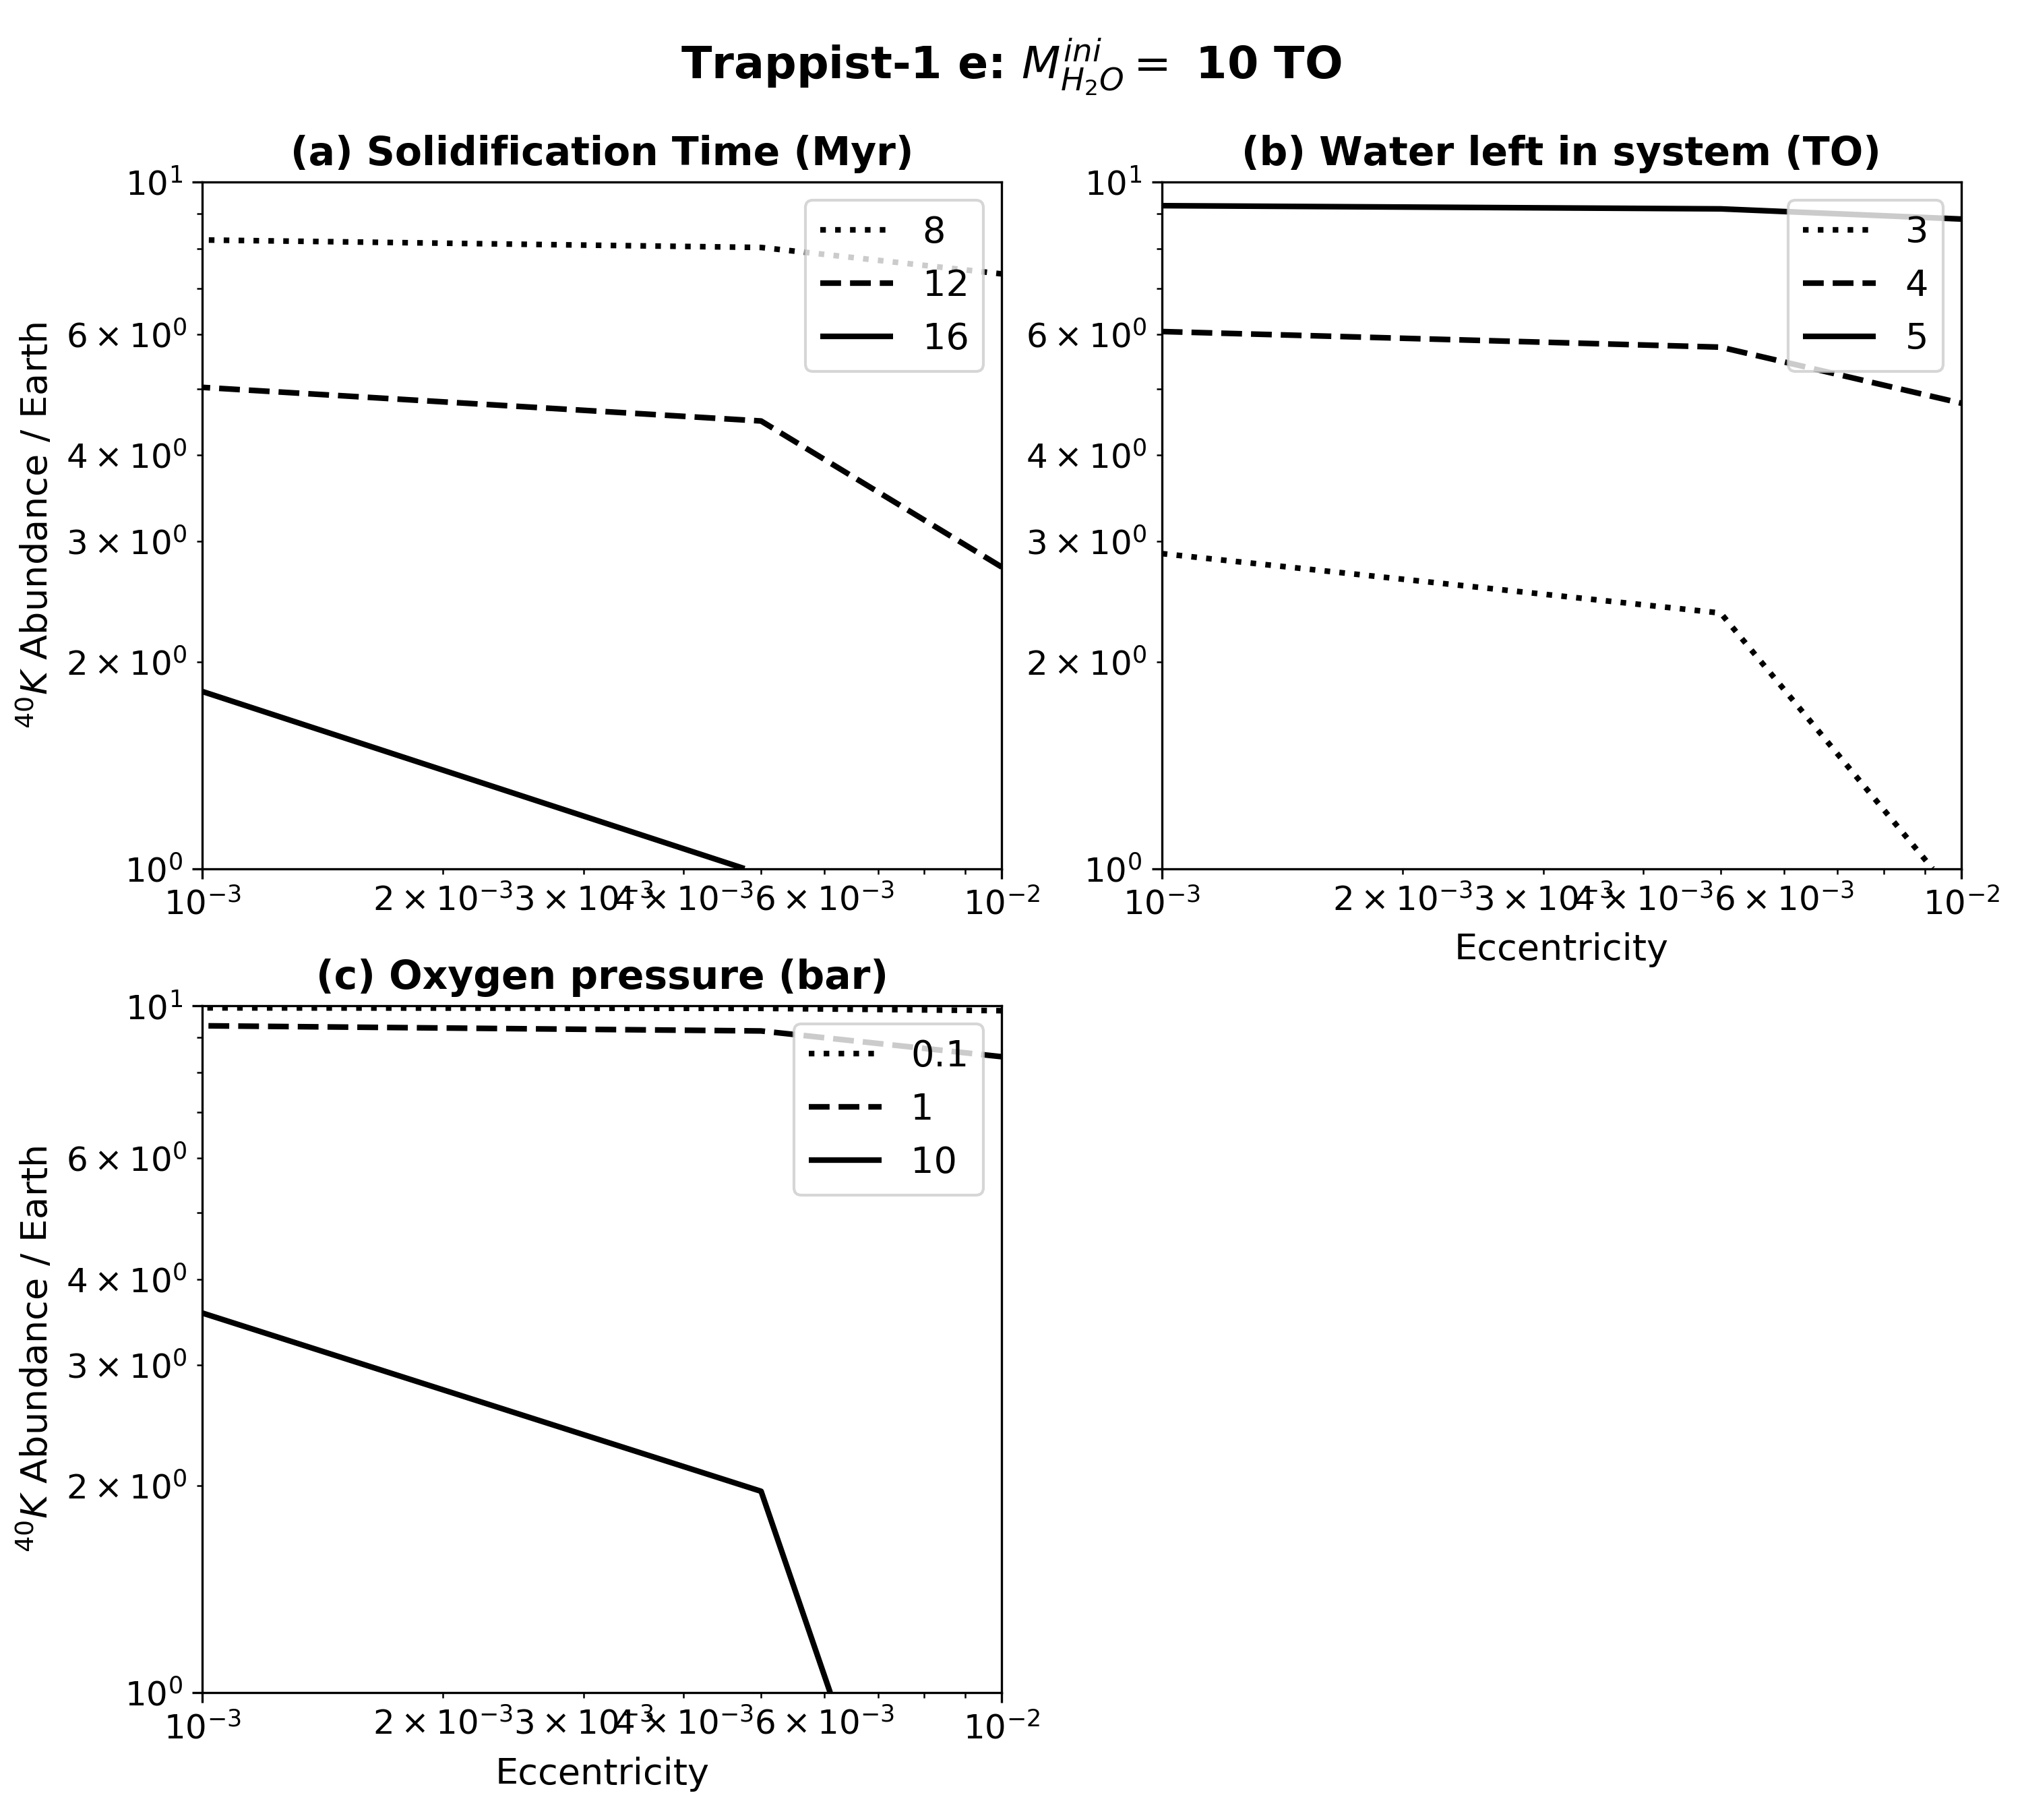
\includegraphics[width=\textwidth]{../Fig_Trappist1e_ContourPlot/Trappist-1_e_10TO_CountourPlot}
	\caption{}
	\label{TR1e-Contour}
\end{figure}

\begin{figure}[H]
	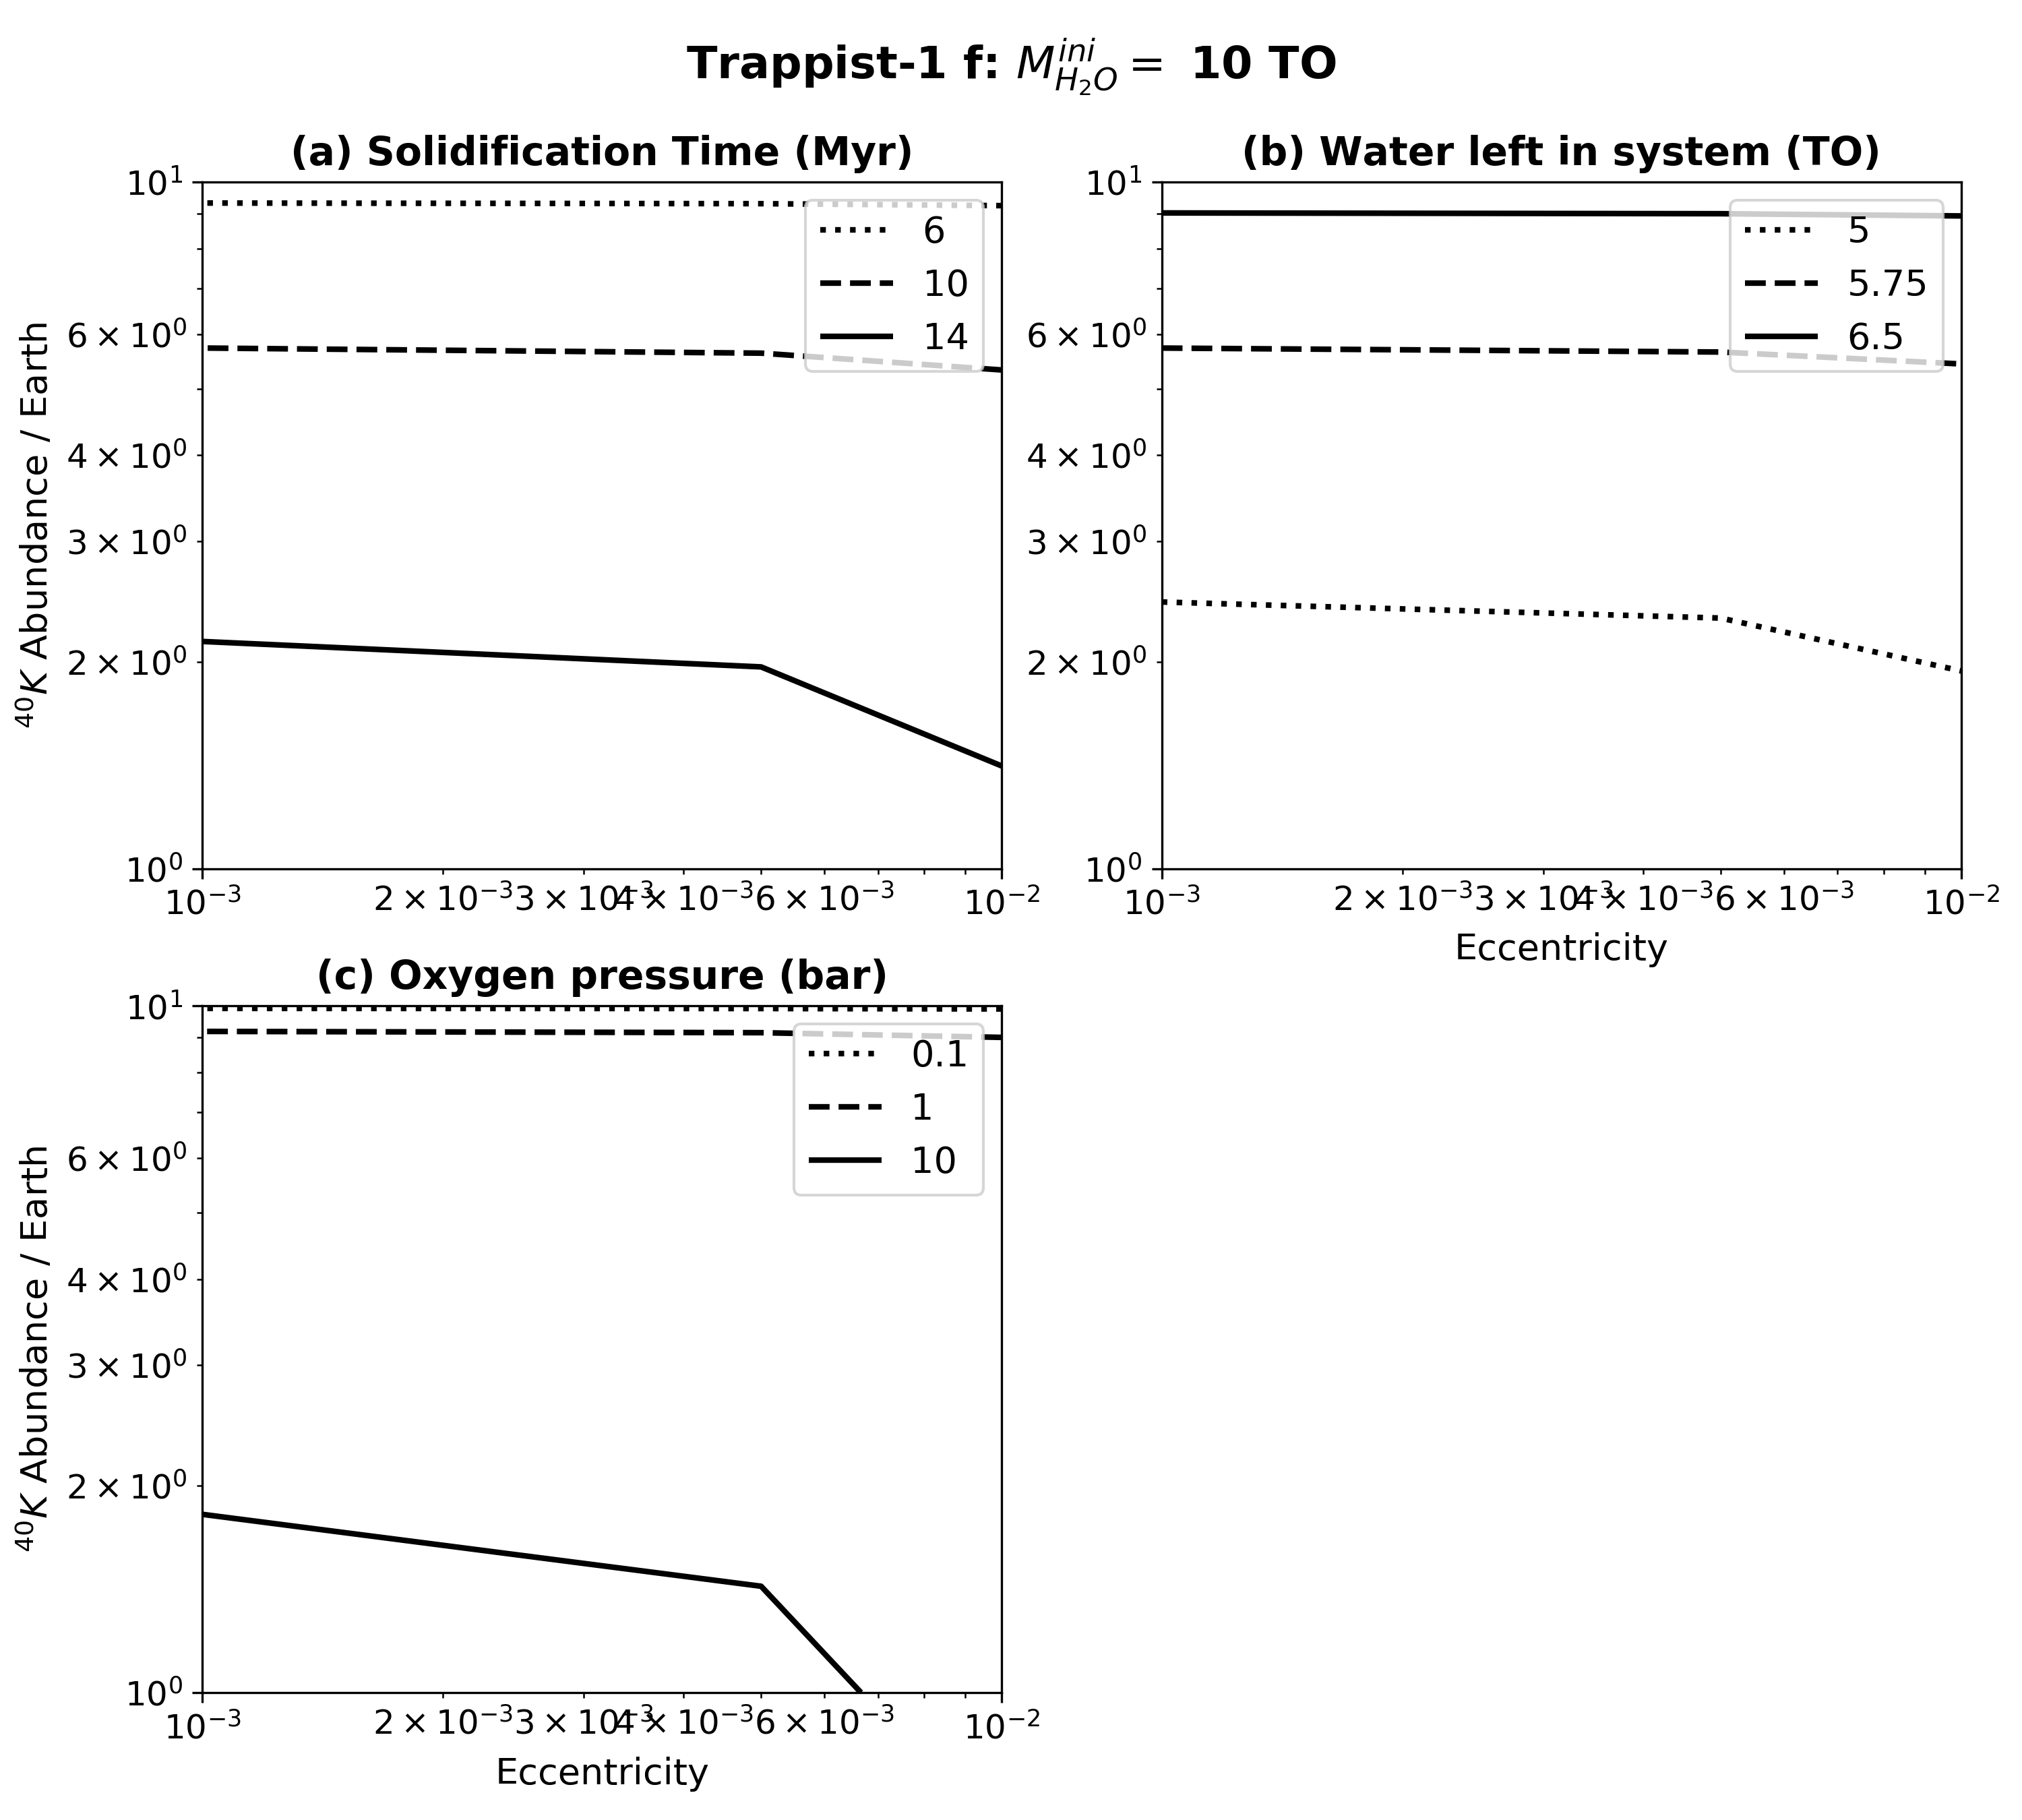
\includegraphics[width=\textwidth]{../Fig_Trappist1f_ContourPlot/Trappist-1_f_10TO_CountourPlot}
	\caption{}
	\label{TR1f-Contour}
\end{figure}

\begin{figure}[H]
	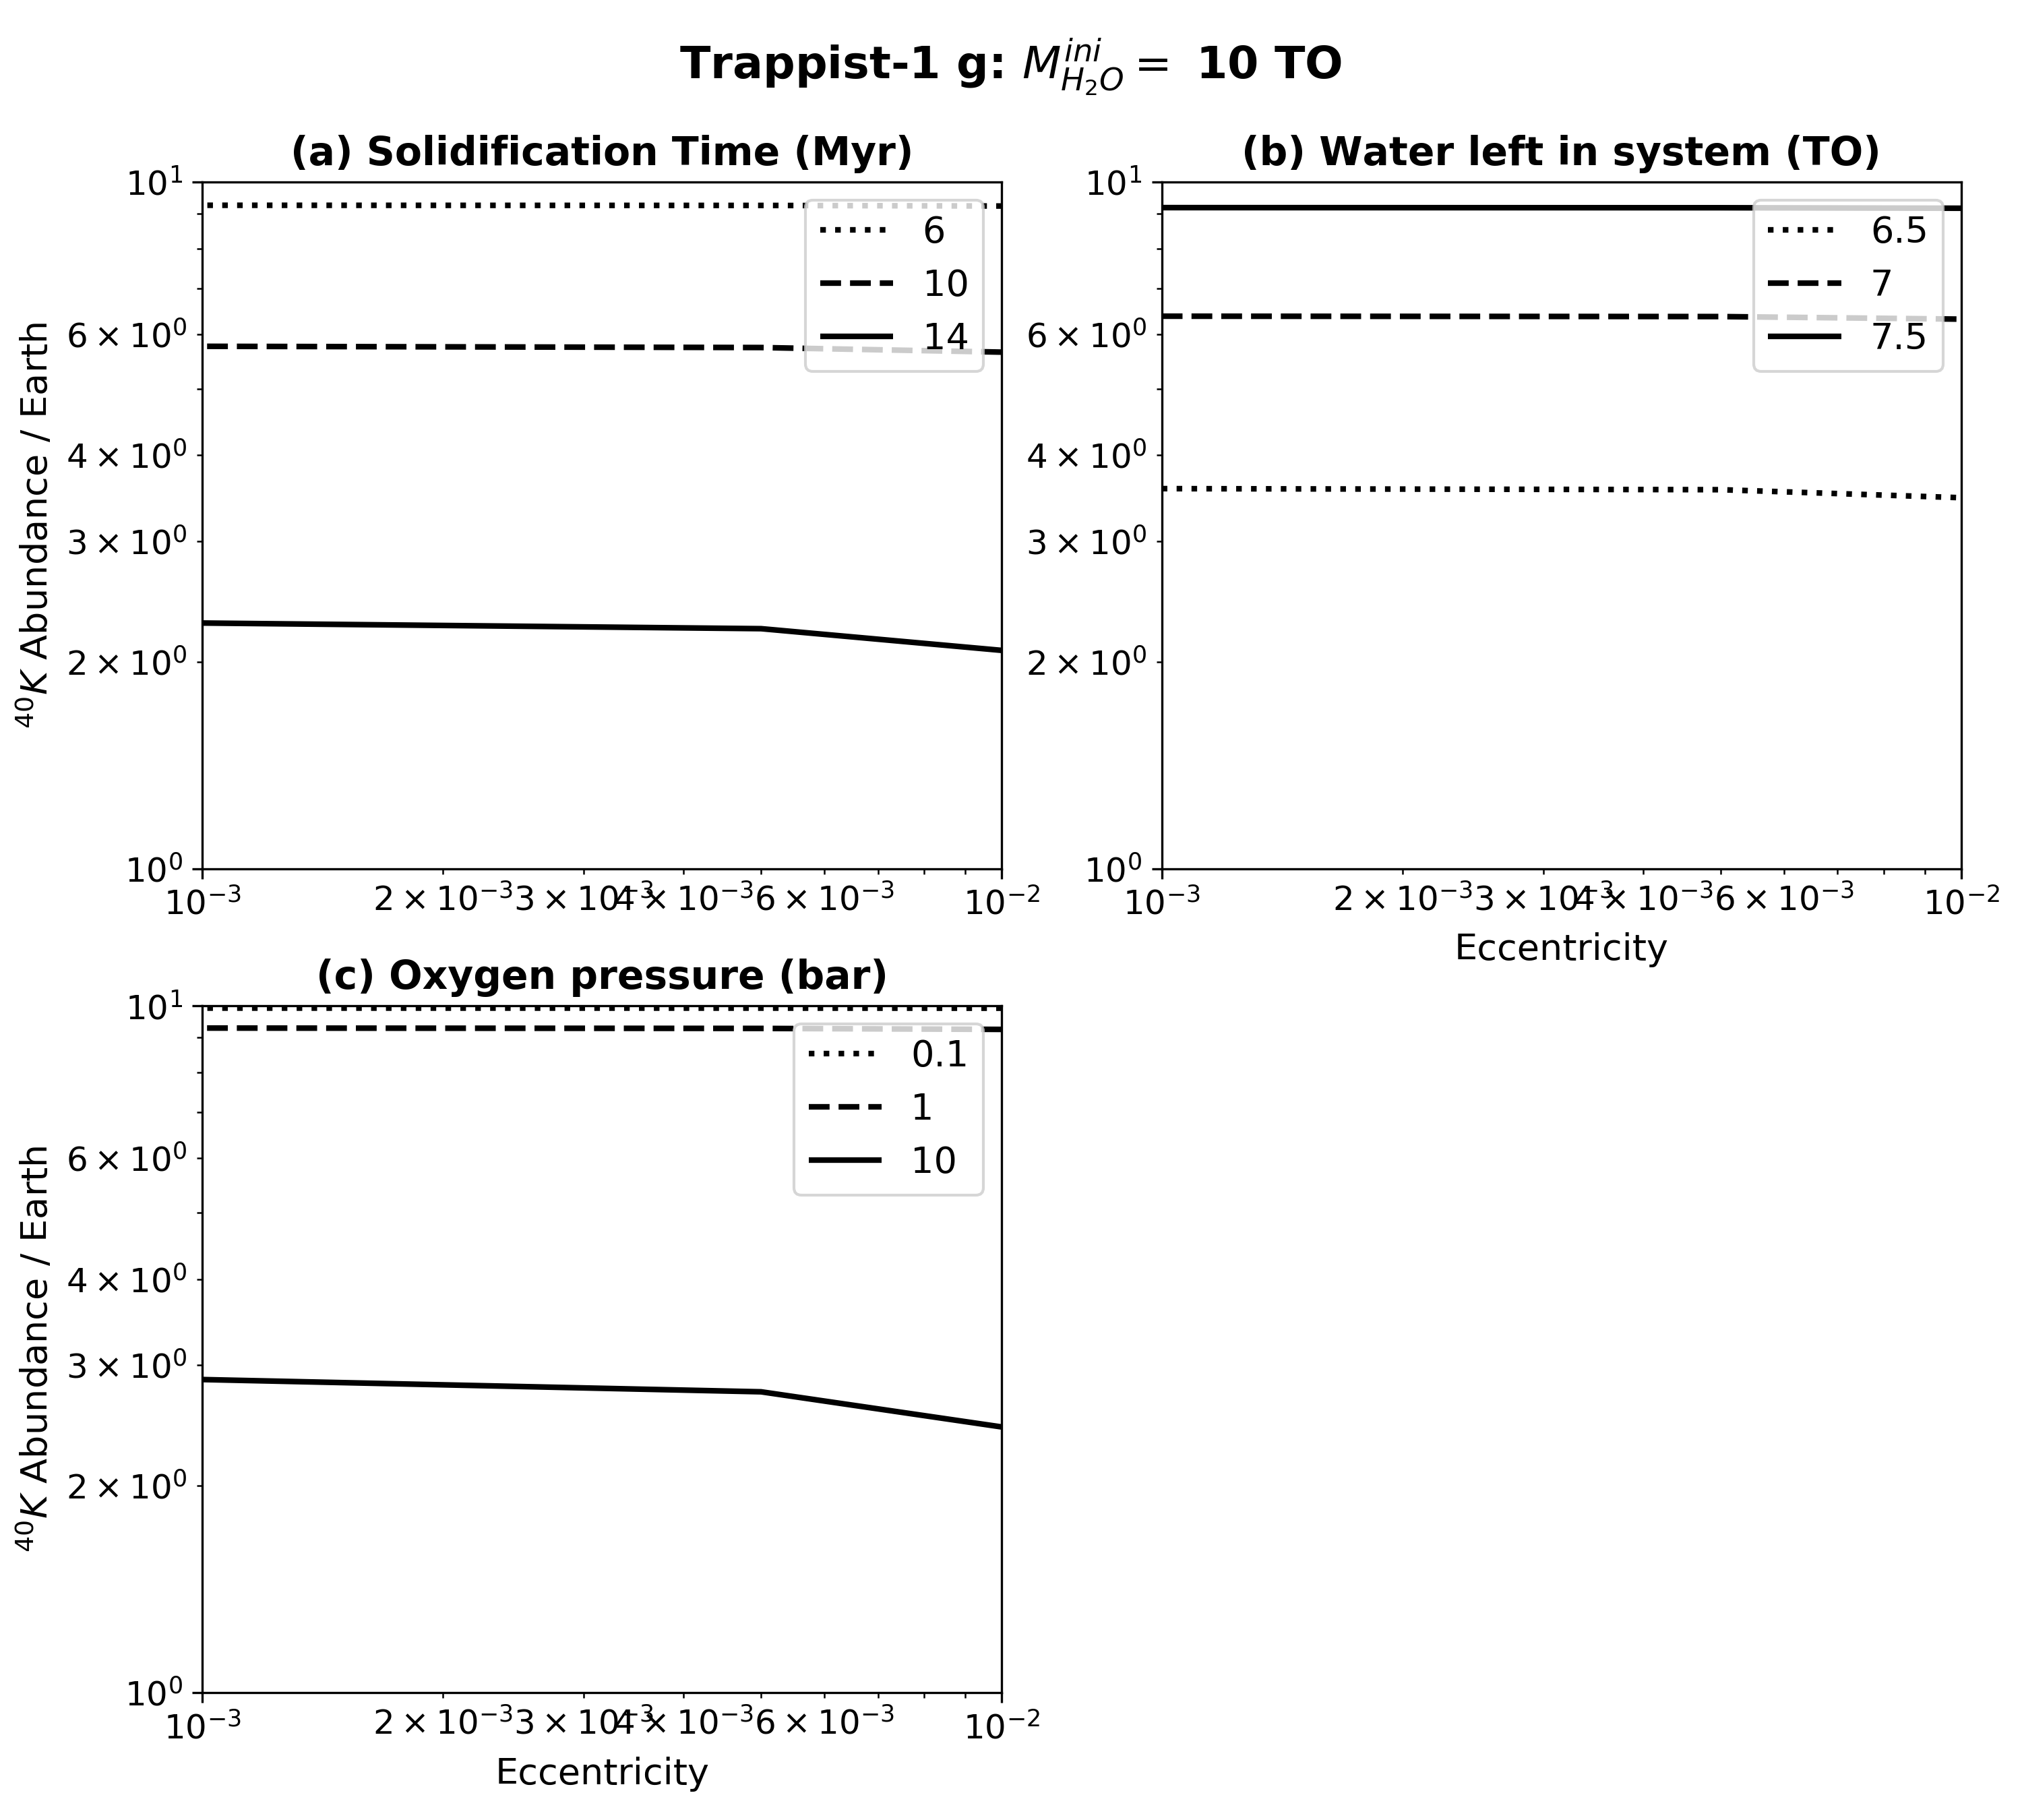
\includegraphics[width=\textwidth]{../Fig_Trappist1g_ContourPlot/Trappist-1_g_10TO_CountourPlot}
	\caption{}
	\label{TR1g-Contour}
\end{figure}

\section{Conclusions}

%\subsection{GJ1132b}

%\begin{figure}[h]
%	\includegraphics[width=\textwidth]{../Results_VPlanet/GJ1132b/MagmOc_AtmEsc/MagmOc_AtmEsc_GJ1132b_N20_100TO_dEta_1_working_log}
%	\caption{Evolution of GJ1132b's magma ocean and volatile inventories for following initial conditions: Initial water mass 100 TO, XUV absorption efficiency $\epsilon_\mathrm{XUV} = 0.3$. Panels from upper left to lower right: Temperature of atmosphere and magma ocean; radius of solidification; water mass in the different reservoirs, atmospheric pressure of water and oxygen, \ce{Fe2O3} mass fraction in the magma ocean; oxygen mass in the different reservoirs (not including oxygen bound in water); number of hydrogen atoms; number of oxygen atoms; change in the total amount of atoms.}
%	\label{GJ1132b_100TO_constTemp}
%\end{figure}
%
%\begin{figure}[h]
%	\includegraphics[width=.8\textwidth]{../Plots/SolidTime_MassFracWater_No5_ConstThermTemp_400K}
%	\caption{Solidification time of GJ1132b's mantle depending on the initial water mass fraction. Results with VPLanet for three different XUV absorption efficiencies (0, 0.15, 0.3) are compared to the results from \citet{Schaefer2016} (Fig. 5).}
%	\label{GJ1132b_SolidTime_constTemp}
%\end{figure}
%
%\subsection{Earth}
%
%In March, I attended the General Meeting of the DFG-SPP 1833 "Building a Habitable Earth" in Cologne, Germany, and presented what I have up to that point in my master thesis.
%Since this meeting was mainly attended by Earth scientists and the main focus was how Earth formed and evolved to a habitable planet I applied my model to Earth.
%The input parameters and settings of the code are summarized in Tab. \ref{Tab_Input_Earth}.
%
%\begin{center}
%	\begin{table}[H]
%		\begin{tabular}{cc}
%			\noalign{\smallskip}
%			\hline
%			\noalign{\smallskip}
%			Symbol & Parameter \\ 
%			\noalign{\smallskip}
%			\hline \hline
%			\noalign{\smallskip}
%			$M_{\ce{H2O}}^\mathrm{ini} $ & 2-20 TO \\
%			$T_\mathrm{surf}^\mathrm{ini} = T_\mathrm{p}^\mathrm{ini} $ & $\SI{4000}{\kelvin}$ \\
%			$\epsilon_\mathrm{XUV}$ & 0.3  \\ 
%			Atmospheric model & grey \\
%			VPLanet modules used & MagmOc, AtmEsc \\
%			\noalign{\smallskip}
%			\hline
%		\end{tabular}
%		\caption{Parameters for the thermal model}
%		\label{Tab_Input_Earth}
%	\end{table}
%\end{center}
%
%\begin{figure}[h]
%	\includegraphics[width=.8\textwidth]{../Plots/Earth_Water_Left}
%	\caption{Water reservoirs on Earth after the solidification of the mantle, normalized to and depending on the initial water mass.}
%	\label{Earth_Water_After_Solid}
%\end{figure}





%----------------------------------------------
\bibliographystyle{plainnat}
\bibliography{../../../../library}

\end{document}